% main.tex
% 北方工业大学本科毕业设计论文 LaTeX 主文件
% 使用 XeLaTeX 编译

\documentclass{ncut-thesis}

% ==================== 参考文献数据库 ====================
\addbibresource{references.bib}

% ==================== 论文信息 ====================
% 封面信息
\titlefirstline{这里是论文的中文题目第一行}    % 题目第一行
\titlesecondline{这里是论文的中文题目第二行}   % 题目第二行
\thesistitle{这里是论文的完整中文题目}  % 完整中文标题
\thesistitleEN{Here is the English Title of the Thesis}  % 英文标题
\studentname{张三}            % 学生姓名
\studentid{22101010000}       % 学号
\classname{某某班级}         % 班级
\department{某某学院}        % 院系
\major{某某专业}     % 专业
\advisor{李四 教授}           % 指导教师
\submitdate{2026年5月}       % 提交日期

\usepackage{pdfpages}

% ==================== 文档开始 ====================
\begin{document}

% ==================== 封面及原创性声明 ====================
% 提示：使用学校给定的 docx 模板填写好封面和声明，然后导出为 PDF，例如命名为 cover.pdf。
% 然后使用 \includepdf 引入（请确保路径正确）。
% 如果要生成纯代码的论文进行测试，可以注释掉此行。
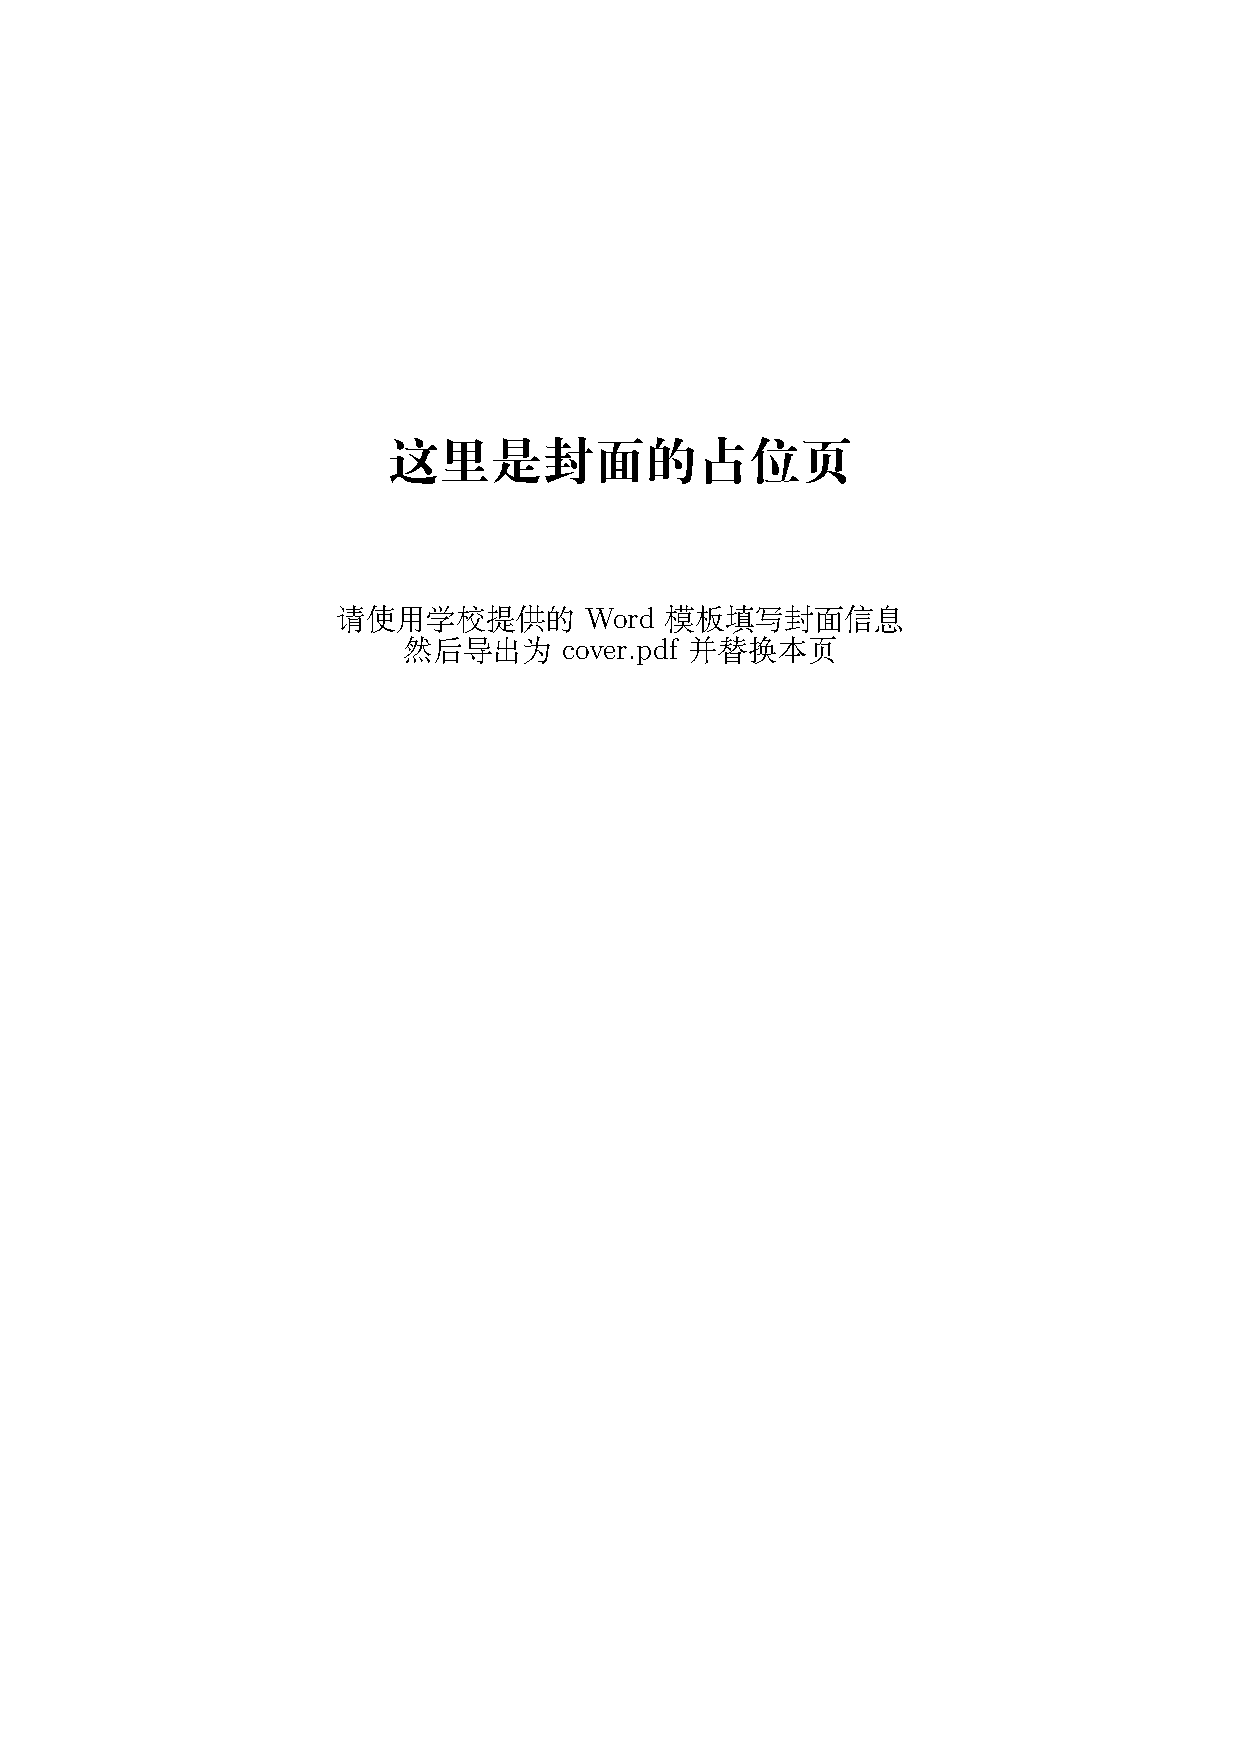
\includepdf[pages={1-2}]{cover.pdf}

% ==================== 前置部分 ====================
\frontmatter
\pagestyle{frontmatter}

% 中文摘要
% abstract_cn.tex
% 中文摘要

\begin{cnabstract}
这里是中文摘要部分。请在这里简要概括论文的研究背景、目的、方法、结果和结论。摘要应具有独立性和自含性，即不阅读论文全文，就能获得必要的信息。摘要中一般不用图、表、化学结构式、计算机程序，也不用非公知公用的符号、术语和非法定的计量单位。摘要内容一般在 300 到 500 字左右。

本文主要研究了某某课题，提出了某某方法，取得了某某成果。这些成果在某某领域具有一定的应用价值和理论意义。

\cnkeywords{关键词1；关键词2；关键词3}
\end{cnabstract}


% 英文摘要
% abstract_en.tex
% 英文摘要

\begin{enabstract}
Here is the English abstract. Please briefly summarize the research background, purpose, methods, results, and conclusions of the thesis here. The abstract should be independent and self-contained, meaning that necessary information can be obtained without reading the full text of the thesis. Figures, tables, chemical structural formulas, computer programs, as well as non-publicly known symbols, terms, and non-statutory units of measurement are generally not used in the abstract. The abstract is generally around 300 to 500 words.

This paper mainly studies the subject of XXX, proposes the method of YYY, and achieves the result of ZZZ. These results have certain application value and theoretical significance in the field of WWW.

\enkeywords{Keyword 1; Keyword 2; Keyword 3}
\end{enabstract}


% 目录
\tableofcontents

% ==================== 正文部分 ====================
\mainmatter
\pagestyle{mainmatter}

% 各章节内容
% chapter1.tex
\chapter{引言}
\label{chap:intro}

\section{研究背景及意义}
这里是第一章第一节的内容。毕业设计（论文）是本科培养计划的重要组成部分。为了规范本科生毕业设计（论文）的撰写，保证论文质量，特制定本模板\cite{rabiner1989tutorial}。

\section{国内外研究现状}
\subsection{国内研究现状}
这里是1.2.1节的内容。引用的相关文献可以放在这里\cite{hinton2012deep}。

\subsection{国外研究现状}
这里是1.2.2节的内容。

\section{本文主要研究内容}
本文的主要研究内容如下：
\begin{itemize}
    \item 第一部分研究了……
    \item 第二部分实现了……
    \item 第三部分验证了……
\end{itemize}

\section{论文组织结构}
本文的组织结构安排如下：
第一章：引言。介绍了研究背景和意义。
第二章：理论基础。
第三章：系统设计。
第四章：实验与分析。
第五章：总结与展望。
   % 引言
% chapter2.tex
\chapter{理论基础与相关技术}
\label{chap:theory}

\section{公式排版示例}
本节展示数学公式的排版方法。行内公式可以直接使用 \verb|$...$| 包裹，例如著名的质能方程 $E = mc^2$。如果是独立的居中公式，应使用 \verb|equation| 环境，如式\ref{eq:emc}所示：

\begin{equation}
    E = mc^2
    \label{eq:emc}
\end{equation}

对于复杂的多行公式，可以使用 \verb|aligned| 或 \verb|gather| 环境：

\begin{equation}
    \begin{aligned}
        \min_{\theta} \quad & \mathcal{L}(\theta) = \frac{1}{N} \sum_{i=1}^{N} L(f_\theta(x_i), y_i) \\
        \text{s.t.} \quad & ||\theta||_2 \leq C
    \end{aligned}
\end{equation}

\section{表格排版示例}
本节展示如何在论文中排版规范的三线表。根据排版规范，表格的表题应位于表格的**正上方**居中，字号为五号黑体。在 LaTeX 中，我们通常使用 \verb|booktabs| 宏包提供的 \verb|\toprule|、\verb|\midrule| 和 \verb|\bottomrule| 来绘制三线表。如表\ref{tab:sample_table}所示：

\begin{table}[htbp]
    \centering
    \caption{示例三线表排版说明}
    \label{tab:sample_table}
    \begin{tabular}{llcc}
        \toprule
        \textbf{序号} & \textbf{测试项目} & \textbf{准确率 (\%)} & \textbf{延迟 (ms)} \\
        \midrule
        1 & 基础模型测试 & 92.5 & 120 \\
        2 & 改进模型A测试 & 95.2 & 135 \\
        3 & 改进模型B测试 & \textbf{96.8} & 110 \\
        \bottomrule
    \end{tabular}
\end{table}

\section{图片排版示例}
本节展示图片的插入方法。根据规范，图题应位于图片的**正下方**居中，字号为小五号黑体。所有图片文件请放置在根目录下的 \verb|figures/| 文件夹中。

这里我们插入一张格式检测的报告截图作为示例，如图\ref{fig:sample_figure}所示。

\begin{figure}[htbp]
    \centering
    % 宽度可以设置为页面宽度的比例，如 0.8\textwidth
    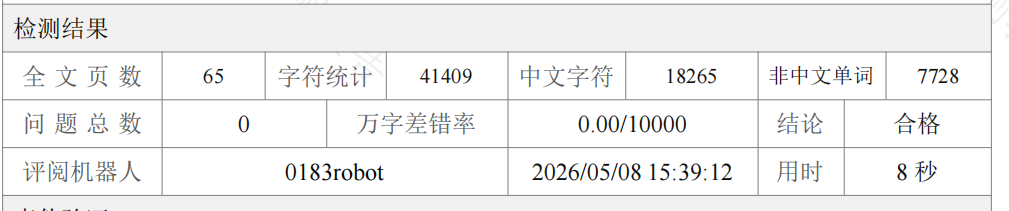
\includegraphics[width=0.8\textwidth]{assets/格式检测结果.png}
    \caption{格式检测系统结果示例图}
    \label{fig:sample_figure}
\end{figure}

如果需要并排插入多张子图，可以利用 \verb|subcaption| 宏包提供的 \verb|subfigure| 环境来实现。

\section{参考文献引用示例}
本节展示参考文献的交叉引用方法。本模板已经集成了基于 \verb|biblatex| 的国标 GB/T 7714-2015 样式宏包，所有的参考文献信息均存储在 \verb|references.bib| 文件中。

\begin{itemize}
    \item \textbf{上标引用}：这是最常用的引用方式，如“在深度学习领域，Hinton等人的研究\cite{hinton2012deep}奠定了基础”。
    \item \textbf{多重引用}：可以同时引用多篇文献，如“语音分离技术经历了快速的发展\cite{luo2019conv, lu2024music}”。
    \item \textbf{作为句法成分（非上标）}：如果文献编号作为句子的一部分，应使用 \verb|\parencite|，如“详细的推导过程可参考文献 \parencite{wang2006computational} 的第三章”。
\end{itemize}

请注意，你只需要在 \verb|references.bib| 中按照 BibTeX 格式填好条目信息，并在文中使用 \verb|\cite|，文末的参考文献列表会自动生成，并且悬挂缩进等格式均符合学校的最新排版要求。
   % 多语种数据构建与评测体系设计
% chapter3.tex
\chapter{系统设计与实现}
\label{chap:design}

\section{系统总体架构}
本章介绍了系统的整体设计思路。

\section{核心模块实现}
介绍了核心模块的具体实现细节。这里可以引用代码环境，如果配置了相应的宏包的话。
   % 多语种语音模型评测实验
% chapter4.tex
\chapter{系统测试与结果分析}
\label{chap:test}

\section{测试环境}
介绍了测试所使用的硬件和软件环境。

\section{测试结果}
展示测试的数据和图表。
   % 语音分离模型评估
% chapter5.tex
\chapter{总结与展望}
\label{chap:summary}

\section{工作总结}
对本文所做的工作进行全面的总结。

\section{未来展望}
指出现有工作的不足，并对未来的改进方向进行展望。
   % 全双工语音对话系统设计与实现

% ==================== 后置部分 ====================
\backmatter

% 致谢
% acknowledgement.tex
% 致谢

\begin{acknowledgement}
这里是致谢内容
\end{acknowledgement}


% 参考文献
\printbibliography[heading=bibintoc, title={参考文献}]

% 附录（可选）
% appendix.tex
% 附录

\begin{appendix}
这里是附录内容。可以放置一些不宜放在正文中，但又具有参考价值的内容。比如推导过程、部分核心代码、或者补充的图表等。

附录格式要求：标题黑体三号居中，内容宋体小四号。
\end{appendix}


\end{document}
